\chapter{重修微积分7——测度}

计量是数学的肇始。无论是称重量,量尺寸,度面积,计体积,结果都是从0到无穷大的一个数。计算时多将整体划分成比较规范的部分,分别测量累加而成。不因测量的方法不同而异。所以计量必须具备几点:它是非负的数量,空无为0,划分后计量之和等于总体,不因测量方法而变。在无限可分世界里任何的计量,就必须把这性质推广到无穷的集合。抽象集合中的\textbf{测度m},就是将集合的子集映射到$ [0,\infty] $区间的函数,空集对应着0,测度有着可数可加性,即:
\begin{equation}
	m(\phi )=0,\;\;\; m(\bigcup_{n=1}^\infty  E_n)=\sum _{n=1}^{\infty} m(E_n),\;\; E_i \cap E_j =\phi\;\;\forall i\neq j
\end{equation}

在不同坐标系下表示集合的点,测度值要保持对坐标变换的不变性。注意,无穷大这里也可以是个测度的量值,这让它适用于一些无穷的情况,比如说没有尽头的直线长度,无边无际的平面面积和无限空间的体积等等。例如,集合的势也是一个测度,满足0的对应和可数可加性,对于有限集,这测度是集合中元素的数量,对无穷集,这测度是无穷大。人们的计数其实是从这个测度开始的。

显然对于同一个集合,可以定义不同含义的测度。学习数学的抽象,这是要适应的思想方法。

这个系列介绍过收敛、拓扑、距离、范数、内积、测度等数学的概念,在集合的基础上定义它们的性质。在同一个基础集合上,往往有多种具体的结构和映射符合这些定义的性质,它们的抽象都属同一概念。这情形与物理等自然科学很不同,让有些学者觉得不习惯和不确定。在思想方法上,自然科学本质是归纳的,研究的都是具体一类的事物,从中抽象发现一些共有的性质,形成了概念。虽然有时用抽象的语言来定义,也因此逻辑推理,但隐在定义之后的具体一类事物,始终是最终的裁判,当推理的结论逸出接受的范围,就放弃原有的概念代之以新的解读。而数学的本质是演绎,虽然许多概念的形成来自归纳,但不同定义的概念在逻辑上必须是一致的,等价的,或是由论域的局限或推广。数学研究的是由这些共同性质定义下的概念,在演绎下的共同表现,不论概念所指的具体对象的类别有多大的不同,所得的结论从具体对象来看会如何不可思议。就抽象所聚焦的概念而言,它们都是一样的,拥有共同推理而得的性质。在数学最高的权威是逻辑而不是事实。所以要构造数学概念的直观图像,必须习惯用多种不同类别的具体对象(在数理逻辑上称之为模型)来想象抽象的概念,了解不同模型的局限,而不要被它所左右。自然科学关心物质世界里的真。数学关心的是思维世界里的真。只有确信思维中逻辑推理的结论是真实可靠的,才能利用数学概念作为工具,来了解、表达和推测物质世界里的真实。

让我们从测度的定义出发,看当逻辑与事实冲突时,数学家和自然科学家的不同处理。

实践经验告诉我们,将一个物体分割成几部分,分别测量它们的重量和体积,它们之和一定会等于整体。这已经成了无可置疑的真理。很不幸,经验不能代替逻辑,因为经验只涉及到有穷的世界,当我们把物体看成无穷可分时,无穷集合的任意分割,并非都能如此。在定义了一些集合测度后的空间里,并非所有的集合都可以参与保有这样性质的测度。

\kaishu\setlength{\leftskip}{1em}

巴拿赫-塔斯基(Banach Tarski)举了一个例子。大致说来,他用分别沿X,Y两轴左转或右转某个特殊的角度(例如$ arccos(1/3) $)的操作,形成包含4种旋转$ a,a^{-1},b,b^{-1} $的运算序列。这些有限步运算序列生成了一个具有无穷个元素的群H。在序列中刨去相邻反向相消的旋转,可以证明每个序列与群H中的元素一一对应。这个群里的元素可以按生成时,第一个的旋转操作分别为$ a,a^{-1},b,b^{-1} $而分成不相交的4组及单位元e组。实心球中的质点,在这群每个元素对应的旋转操作序列作用下,形成一条旋转轨迹质点相连的链。利用选择公理,在每个链条都可以选出一个点来代表,这些点的集合记为M,球中所有的质点都在M中某点所在的轨迹链条中。这些轨迹链条依对应的4个群组也分成4组,将这些轨迹链条的第一个质点取出放在对应于群的e组,其余链条中的质点对应到起始旋转分别为$ a,a^{-1},b,b^{-1} $的群组,它们是互不相交的5个组,可以看成球被分割成5堆。现在将对应$ a^{-1} $组那堆整体做a的旋转,经过这旋转后的这堆包含有对应着所有$ a^{-1},b,b^{-1} $组及部分e组的质点,对$ b^{-1} $组那堆整体做b的旋转,得到类似的结果,不难想象将它们与剩下的a,b和e组可以组装成没有缝隙与原来一样的两个球,详见【2】。

这个例子很有名,称为``分球悖论''或者``巴拿赫-塔斯基定理'',因为进行分类时,用了选择公理(AC)在无穷集合中挑选,上世纪二十年代,大家是用来反对AC的。经过多年争论后,人们发现这里的证明在逻辑上无懈可击,选择公理在数学基础上很重要,是必须保护的不可或缺。而在物质世界中球不可能由无限的质点组成,所以这模型并不与现实冲突。想要继续应用抽象的测度理论,那么只能归结为人们在无穷的世界里的直觉错了。

\songti\setlength{\leftskip}{0em}

为什么是不可思议?因为人们觉得将一个球切碎分割成5堆,组成球的元素分成了5个集合,球的重量和体积是这5个集合的总和,一堆元素刚性旋转不会改变重量和体积,即使装配成的球没有缝隙,它们也不该有两个球的重量和体积。

重量和体积都是测度,与经验的冲突在于这种分割不满足可加性。但如果这种怪异分割而成的5个集合是不可测度的,那么就没有理由说什么可加性了。一个球和两个球之间就失去了这个有限测度量的联系。至于一个球和两个球的元素数量,因为它们都是无穷的集合,在有限的世界对岸,集合论早就告诉我们,无穷集合和两倍的集合,它们的元素是可以一一对应的。这例子告诉我们,测度有时只能定义在空间的一部分集合上,这些集合称为\textbf{可测集},它们包括空集,对可数个并,及补集运算封闭,称为$ \mathbf{\sigma} $\textbf{代数}。在这$ \sigma $代数之外的集合,对测度没有定义,称为不可测集。

在实数空间,我们定义开区间$ (a, b) $的测度为$ |b-a| $,以开区间生成的$ \sigma $代数称为\textbf{波雷尔(Borel)集}。在实数空间以开区间测度和定义延拓出来的测度称为长度。在n维欧几里德空间,可以同样地从定义矩形区间的面积延拓出2维的测度,以及n维的体积,这样定义的测度称为勒贝格测度。在不致混淆时,简称为测度,或长度、面积、体积。

波雷尔集包含着$ \mathbb{R}^n $空间通常拓扑下的所有空集、全体、开集、闭集、单点、以及它们的各种交和并。在理论上,不可测的集合虽然也有无穷多,你可以想象的却很难,因为它们不存在你的经验中,它必须用逻辑依赖选择公理来构造。

柯尔莫哥洛夫将公理化概率论定义在概率空间上,用样本的集合代表事件,它们构成空间里的$ \sigma $代数,概率则是对集合取值在0到1之间的测度。

测度为0的集合叫做\textbf{零测集},它在应用中扮演了重要的角色,比如说你突然有个天才的发现,只是它适用的情况在参数中是零测集,如果参数值是随机分布的,那你几乎都没有用武之地。在积分里,如果引起麻烦的地方,比如说无界、间断处等等是零测集,那也可以忽略它们。

$ \mathbb{R}^n $空间中的一个点的集合,可以包含在任意小的区间里,它的勒贝格测度小于任何正数,所以它只能为0。从测度的定义可知,可数个零测集的并集仍然是零测集,所以有理数集合是实数空间$ \mathbb{R} $上的零测集。

有个古老的疑问:``点没有长度,为什么它们组成线段却有了长度?''有人回答,因为这里的点有无穷多,0乘无穷大可以是非零的数。上面例子说明,这理由对可数多的无穷大不成立。是不是因为线段有不可数的点所致?下面例子说明,在直线上不可数点集的总长度也可能是零。

\kaishu\setlength{\leftskip}{1em}

康托集是这样构造的,记$ C_0=[0,1] $,将这区间三等分,取走中间一块$ (1/3, 2/3) $,留下的部分$ C_1=[0,1/3]\cup[2/3,1] $;分别在留下的区间$ [0,1/3] $及$ [2/3,1] $中,再次取走各区间中间$ 1/3 $的那块,得到$ C_2 $;如此重覆得到$ C_n $,$ n=0,1,2,\cdots $;它们的极限C称为康托集。C是不可数的,因为它的点必须选自无穷序列Cn中左边或右边部分,即2的可数幂。$ Cn $测度是$ (2/3)n $,当n趋向无穷大时,它趋向0,所以C的勒贝格测度是0.

\songti\setlength{\leftskip}{0em}

当一个区间无穷地缩小到一个点,区间的长度也无限地趋向0,区间的长度和覆盖线段的区间数总在有限世界这一边,没有尺寸的点和无穷多个点是在实无穷的彼岸,我们不能指望用点和点数来解答线段长度的问题。不同维数空间中几何体的测量也是如此。看个例子。

\kaishu\setlength{\leftskip}{1em}

英国人很早在测量海岸线长度时,发现所用的尺度越短,海岸线的长度越长,那么到底什么是曲线的长度?二维空间的曲线,显然不能用一维区间来覆盖,而二维的勒贝格测度(面积)是零。实践中用尺子丈量曲线,微积分里用折线来逼近曲线长度,都是用二维空间的园来覆盖曲线,然后计算这些覆盖直径的和。对于不同覆盖所计算的下确界,称为曲线的长度。测量所用的尺子越短,计算出来的长度越长,这反映了近似逼近的过程。这个单调递增的数列极限可能是有限的量,也可能是无穷大。

\songti\setlength{\leftskip}{0em}

在n维欧几里德空间,任何集合A都可以被一族可数的开集覆盖,这族开覆盖测度和的下确界称为集合A的外测度,记为$ m^{*}(A) $。外测度对所有集合都有定义,保持有测度的非负性,对集合包含关系的单调性,和次可数可加性。当集合A是可测时,外测度等于它的测度。
\[m^*(A) \ge 0, \; m^*(\phi)=0,\;\;\; A\subset B \Rightarrow m^*(A)\le m^*(B),\]
\[m^*( \bigcup _{n=1}^\infty  E_n) \le \sum _{n=1}^\infty m^*(E_n),\;\; E_i\cap E_j = \phi\;\;\forall i\neq j\]


将开集的测度定义为集合中两点距离的上确界,我们就由此定义了曲线的长度。在有界的二维区域里的曲线长度有没有可能是无穷大?当然有。下面是一个分形曲线的例子。

\kaishu\setlength{\leftskip}{1em}

Koch曲线是这样构造的。对单位线段,中间1/3用等边三角形的两边来代替,得到四条边的曲线k=1,对这四条边做同样的替换,得到k=2曲线,如此无限重复这个替代过程,它趋向Koch曲线。(见图,图像抄自网络)

\begin{figure}[h]
	\centering
	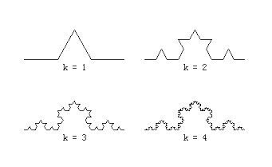
\includegraphics[width=0.7\linewidth]{pic/151409kzeswb2kzreg87zm.png}
	\caption{分形曲线}
	\label{fig:151409kzeswb2kzreg87zm}
\end{figure}


可以把这个k序列看作测量尺度变小的过程,计算不同k时计算的曲线长度$ L(K)=(4/3)^{K} $,所以Koch曲线的长度是无穷大。

\songti\setlength{\leftskip}{0em}

对于欧几里德空间$ \mathbb{R}^n $中的几何体,集合A的\textbf{Hausdorff测度}$ H^s(A) $定义如下:
\begin{equation}
	H_d^s(A)=\inf \left\{\sum_{i=1}^\infty |O_i|^s \mid \bigcup_{i=1}^\infty O_i \supset A, \;\; |O_i| \le d\right \},\; 
	H^s(A)=\lim_{d\rightarrow 0}H_d^s(A)
\end{equation}

$H^s(A) $定义在$ \mathbb{R}^n $的Borel集上,不难验证它满足可数可加性,所以是个带参数s的测度。当s=n时,$ H^s(A) $是$ \mathbb{R}^n $的n维勒贝格测度(精确地说只差一个与n有关的倍因子,因为Hausdorff测量的尺子是球,勒贝格是方块)。

在$ \mathbb{R}^n $空间,将几何体A线性放大k倍,其集合记为$ kA =\{kx \; | \; x\in A\} $,则有 $ H^s(kA)=k^sH^s(A) $,这与k维几何体的线性放大后,长度、面积和体积比例关系是一致的。注意到对于给定的集合A,Hausdorff测度$ H^s(A) $,随着s从n+1开始减小,其数值从0,到了一个临界点后,突然跳到无穷大,我们把这个s的临界值,称为几何体的维数,或者\textbf{Hausdorff维数}。当它是自然数时,这与我们日常中的经验是一致的,但有时它不是一个整数。

作为一个应用的例子,现在我们审视$ \mathbb{R}^n $空间里曲线的长度,凡是能够用积分算出有限值长度的,无论在平面或在三维空间,用Hausdorff测度可以证明都是一维的曲线。Koch曲线按照s=1来计算是无穷大,所以它可能是更高的维数。分形物体具有自相似结构,注意到如果将Koch曲线线性放大3倍,可以得到4份的原来曲线,根据上述s维几何体的线性放大与Hausdorff测度的倍数关系,可以算出$ s=ln4/ln3=1.26186... $,即Koch曲线是1.26186...维。前面例子中的康托集,线性放大3倍可以得到2份原来的康托集,所以它的维数是$ s=ln2/ln3=0.63093... $,是分数维的。只有在几何体所在的维度里的测度,才可能是一个正实数值。

如果你好奇,$ \mathbb{R}^n $空间里一个点的维数是多少?建议你用Hausdorff测度公式验算一下,以加深理解。只有s=0时,单点的Hausdorff测度是1,k个点和可数无穷个点,测度是k和无穷大,而它们在s>0时都是零测集。不可数的点集,在s=1时的测度,既可能为0,如康托集;也可能是正数,如有界区间;也可能是无穷大,如整条直线;还可能没有定义,如不可测集。这也许能给予古老的点与线段长度关系问题,更多一点的认识。

【扩展阅读】
\begin{enumerate}
	\item 维基百科,测度
	\url{http://zh.wikipedia.org/wiki/\%E6\%B5\%8B\%E5\%BA\%A6}
	
	\item  Wikipedia,Banach–Tarskiparadox \url{http://en.wikipedia.org/wiki/Banach\%E2\%80\%93Tarski_paradox}
	
	Wikipedia,Hausdorffmeasure 
	\url{http://en.wikipedia.org/wiki/Hausdorff\_measure}
	
	\item 维基百科,维塔利集合
	\url{http://zh.wikipedia.org/wiki/\%E7\%BB\%B4\%E5\%A1\%94\%E5\%88\%A9\%E9\%9B\%86\%E5\%90\%88}
	
\end{enumerate}
